
\section{Analisi e riconciliazione delle sorgenti operazionali}
Dati i Database sorgenti è necessario studiarli e analizzarli per capire come effettuare l'operazione di riconciliazione.\newline
In output avremo lo schema riconciliato e il mapping.
Ogni attributo dello schema sorgente è infatti collegato in qualche modo allo schema riconciliato.\newline
Per effettuare analisi e riconciliazioni in generale è sufficiente conoscere la struttura degli schemi, e non sapere come sono fatti i dati.\newline
Quando invece servirà effettuare l'operazione di cleaning e di trasformazione serviranno anche le forme dei dati.
\begin{figure}[H]
	\begin{center}
		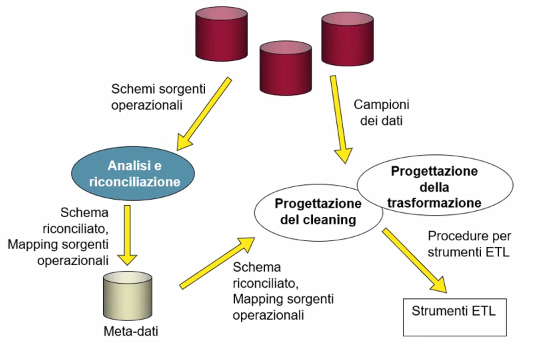
\includegraphics[width=0.6\linewidth]{img/riconciliato.PNG}
		\caption{Riconciliazione degli schemi sorgente}
	\end{center}
\end{figure}
\noindent Di ciascuno schema sorgente è necessario effettuare un'operazione di ricognizione e di normalizzazione, qualora lo schema non sia già normalizzato. Questo accanimento sulla normalizzazione è dovuto al fatto che l'algoritmo per fare la progettazione concettuale del Data Mart funziona attraverso le dipendenze funzionali. Se la normalizzazione non c'è l'algoritmo non funziona bene e restituisce risultati sbagliati, perché alcune dipendenze funzionali non sono visibili.\newline
Una volta che tutti gli schemi sono normalizzati si possono integrare gli schemi. In output avrò uno schema concettuale globale riconciliato. Questo schema è a tutti gli effetti lo schema concettuale dell'ODS.\newline
\begin{figure}[H]
	\begin{center}
		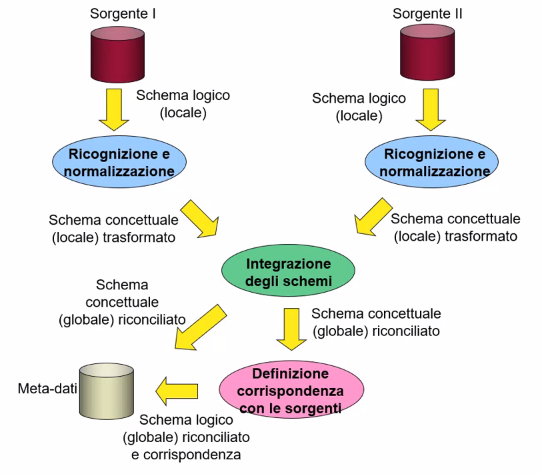
\includegraphics[width=0.5\linewidth]{img/integration.PNG}
		\caption{Integrazione degli schemi sorgenti}
	\end{center}
\end{figure}
\noindent Il processo di integrazione non è semplice. Esistono diversi tipi di architetture. Può essere un'attività particolarmente lunga perché non esistono automatismi.

\subsection{Analisi dei Requisiti}
L'obiettivo è raccogliere i requisiti dagli utenti finali. Gli scopi sono prendere decisioni su diversi ambiti:
\begin{itemize}
	\item sullo schema concettuale dei dati;
	\item sul progetto dell'alimentazione;
	\item sulle specifiche delle applicazioni;
	\item sul piano di avviamento e sulla formazione;
	\item sulle linee guida per la manutenzione e l'evoluzione.
\end{itemize}
Le fonti sono gli utenti di business, ma anche figure più tecniche come gli amministratori del sistema informativo e/o i responsabili del CED.

Le interviste con gli utenti possono essere di due tipi:
\begin{itemize}
	\item \textbf{A piramide}: L'approccio utilizzato è induttivo, si parte da domande dettagliate per poi ampliare l'argomento con domande più generali. L'intervistato scettico potrebbe sorpassare la fase di riluttanza.
	\item \textbf{A imbuto}: L'approccio utilizzato è deduttivo, si parte da domande generali per poi restringere su temi specifici. L'intervistato potrebbe sentire meno tensione.
\end{itemize}
L'approccio dipende fortemente dall'intervistato. Quando l'utente si trova a dover raccontare i suoi problemi non riesce a centrare il punto della questione, un bravo intervistatore non deve lasciarlo uscire dai binari, ma neanche interrogarlo e basta.\newline
Le domande vanno fatte anche in base al tipo di intervistato e al suo ruolo all'interno dell'azienda.
A volte dei questionari con domande preimpostate può aiutare gli utenti a fare mente locale e a non sbagliare.\newline
Lo scopo dell'analisi dei requisiti resta identificare i fatti. Importante è capire qual è il livello di \textbf{granularità} necessario da mantenere. Alcuni dettagli potrebbero essere di interesse per l'azienda, altri no. Serve un compromesso su quali dati sono importanti e quali no. Mantenendo un livello di dettaglio troppo alto il cubo avrà dimensioni troppo onerose (tanto spazio significa anche tanto tempo per eseguire query) mentre rimuovendo dettagli si perdono potenziali informazioni utili.\newline
Per ogni fatto occorre anche definire l'intervallo di storicizzazione, ovvero l'arco temporale che gli eventi memorizzati dovranno coprire. Una soluzione può essere creare due cubi, uno più dettagliato che copre un periodo temporale più breve e uno più aggregato che copre un periodo più lungo.\newline
Il carico di lavoro preliminare influenza pesantemente il riconoscimento dei fatti dimensioni e misure.\newline
Non dovremmo preoccuparci di quali query riusciamo a formulare perché l'approccio utilizzato per creare il Data Mart ci porterà alla possibilità di creare una quantità veramente notevole di query, anche alcune a cui l'utente non penserebbe ma che in realtà potrebbe ritenere utili.\newline
